\chapter{Asking Houston Moguls How They Got Rich!}

This chapter follows a School of Hard Knocks street interview, curated by LazyingArt LLC, in which Houston is treated as a field of concentrated wealth and the city itself becomes part of the argument. The lecture does not give us a single theory of riches. It gives us a sequence of commercial mechanisms in the order in which the host encounters them: healthcare concentration, problem-solving, faith and personal brand, sponsor arithmetic about online reach, capital improvisation under stress, and finally the lean cost discipline that makes later scale possible. We will keep that order, because the lecture is built by movement, interruption, recap, and return.

\section{Cold Open and Houston as a Wealth Field}

The lecture opens in a characteristic way: it spends consequence before it spends explanation. We hear fragments of later outcomes first,
\begin{equation}
Y_{\text{cold-open},1} \approx \$4.3\,\text{million},\qquad
Y_{\text{cold-open},2} \approx \$1.7\,\text{million},\qquad
Y_{\text{cold-open},3} \approx \$16\,\text{million},
\end{equation}
together with an age marker,
\begin{equation}
a_{\text{cold-open}} \approx 51,
\end{equation}
and even a teaser question about becoming a billionaire. At this stage we do not yet know who belongs to which number. That is deliberate. The lecture wants the city to feel charged with latent scale before it tells us how that scale is produced.

Only then does the host widen the frame. Houston is introduced not as generic scenery but as a dense wealth field:
\begin{equation}
N_{\text{millionaires}} \approx 100{,}000,\qquad
N_{\text{billionaires}} = 18.
\end{equation}
Those numbers are not a theorem; they are the lecture's setup. They justify the method of the day: walk the city, stop operators, and ask them to convert biography into doctrine.

This opening matters for the notes because it tells us how to read everything that follows. We are not in a classroom with one carefully chosen speaker. We are in a search process. The city is the first object of study, and the interviews are the local probes.

\section{The Chiropractor: Risk, Concentration, and the Value of Problems}

The first stable case is a chiropractor. He says he has been in medicine for thirty years and an entrepreneur for eighteen:
\begin{equation}
T_{\text{medicine}} = 30\ \text{years},\qquad
T_{\text{entrepreneur,chiro}} = 18\ \text{years}.
\end{equation}
When asked about the biggest risk of his career, he answers with a plain entrepreneurial line: opening his own business. That is the individual side of the story. The structural side appears immediately afterward when he says the biggest challenge is insurance companies.

Here the lecture becomes more numerical. The chiropractor gives a stock-price example to illustrate how insurer power has grown:
\begin{equation}
P_{\text{UNH},2010} = \$33,\qquad
P_{\text{UNH},\text{now}} = \$213.
\end{equation}
If we simply compute the ratio of the two stated figures, we obtain
\begin{equation}
\frac{P_{\text{UNH},\text{now}}}{P_{\text{UNH},2010}}
= \frac{213}{33}\approx 6.45.
\end{equation}
That number is note-writer arithmetic, not the speaker's own formula. But it is useful because it shows the scale of the price change he is trying to point to.

He then reframes the same complaint in concentration language. Over his career, he says, the insurance industry consolidated from ``20-something'' HMOs and PPOs down to five. The safest cleaned note form is
\begin{equation}
N_{\text{payors,early}} > 20,\qquad
N_{\text{payors,late}} = 5.
\end{equation}
Of those five, Blue Cross is not publicly traded, while the other four are:
\begin{equation}
N_{\text{public payors}} = 4.
\end{equation}
The same speaker then adds a compensation claim:
\begin{equation}
Y_{\text{CEO}} \approx \$100\,\text{million/year}.
\end{equation}
We should keep all of this speaker-attributed. The lecture is not independently verifying the healthcare system. It is showing us how an operator inside that system explains his own pressure.

\begin{figure}[h]
\centering
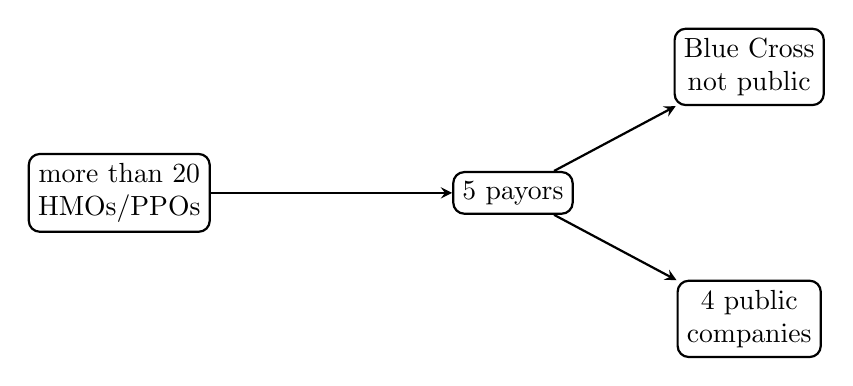
\begin{tikzpicture}[>=stealth,thick]
\node[draw,rounded corners,align=center] (a) at (0,0) {more than $20$\\ HMOs/PPOs};
\node[draw,rounded corners,align=center] (b) at (5,0) {$5$ payors};
\node[draw,rounded corners,align=center] (c) at (8,1.6) {Blue Cross\\ not public};
\node[draw,rounded corners,align=center] (d) at (8,-1.6) {$4$ public\\ companies};
\draw[->] (a)--(b);
\draw[->] (b)--(c);
\draw[->] (b)--(d);
\end{tikzpicture}
\caption{Transcript-derived schematic of the chiropractor's insurer-consolidation story.}
\end{figure}

The lecture then returns from structure to practice. Asked about the most money he ever made in a year, he says
\begin{equation}
Y_{\text{chiropractor,max}} \approx \$1.7\,\text{million}.
\end{equation}
Asked how he scaled to seven figures, he gives the line that becomes the section's real doctrine:
\begin{equation}
\text{solve wants or needs} \;\Rightarrow\; \text{success},
\qquad
\text{solve problems} \;\Rightarrow\; \text{wealth}.
\end{equation}
This is not a literal board equation from the lecture; it is the clean mathematical form of what he says. It is also the first place where the lecture truly differentiates levels of commercial value.

\subsection{Question \& Answer}

\paragraph{Question.} Why does solving problems create more wealth than merely satisfying wants?

\paragraph{Answer.} Because the lecture is drawing a distinction in depth and urgency. Wants can produce revenue; needs can produce stable demand; but real problems create pressure, and pressure is what makes a customer tolerate price, search, and switching costs. In the lecture's own compressed logic, wealth appears where the operator removes a bottleneck rather than merely offering something pleasant. The point is directional, not absolute, but it is one of the lecture's strongest local ideas.

Before moving on, the host performs an important recap. He restates the chiropractor's line in compressed form: solve wants and needs, and one may become rich; solve problems, and one may become wealthy. These recap beats matter because they tell us what the interview was for.

\section{The Digital-Marketing Founder: Faith, Debt, Real Estate, and Brand}

The next long case begins with another street stop, this time framed by a Lamborghini. The speaker says she runs a digital marketing company, has been a business owner for twelve years, and in her best year made about
\begin{equation}
T_{\text{owner,digital}} = 12\ \text{years},\qquad
Y_{\text{digital,max}} \approx \$4.3\,\text{million}.
\end{equation}
Like the chiropractor's case, this one moves quickly from endpoint to mechanism. But the mechanism is very different.

She says she did not come from a great deal of money, describes a difficult background without naming it as outright poverty, and insists that faith is central to her life and business. The lecture does not give us a numerical faith model, nor should we pretend it does. What it does give us is sequence: hardship, faith, work, then scale.

The turning point she names is graduation from Howard University with dual degrees in business and communications, together with the shock of large student debt:
\begin{equation}
D_{\text{student loans}} \approx \$150{,}000.
\end{equation}
This is a useful number in the lecture because it reminds us that education here is not narrated as a frictionless ascent. It is narrated as a threshold crossed with heavy debt attached.

The strongest doctrinal part of her segment comes when the host asks whether she is a buyer or a seller. Instead of answering with a simple identity, she gives a filter. Many people, she says, treat renting as obviously inferior. She does not. Her concern is equity, cash flow, and whether the thing purchased is actually a good investment:
\begin{equation}
\text{goal} = \text{equity building},
\qquad
\text{buy only if } \text{cash flow} > 0.
\end{equation}
The most compact note form of her real-estate philosophy is
\begin{equation}
\text{rent where you live},\qquad
\text{own what you can rent}.
\end{equation}
We should be careful here. The lecture is not giving a universal anti-homeownership theorem. It is giving us a practitioner's screen: do not buy simply because ownership sounds virtuous; buy where the economics actually work.

That same speaker then shifts from assets to distribution. What helped her stand out, she says, was personal brand. People buy into the person and then into the product. One should not read this as empty self-promotion. In the architecture of the lecture, brand is being treated as a mechanism for lowering social friction in sales.

\subsection{Question \& Answer}

\paragraph{Question.} Can renting be rational inside a serious wealth-building strategy?

\paragraph{Answer.} According to this lecture, yes. The point is not to worship renting or ownership. The point is to separate personal residence from investable asset. If the residence does not pass the cash-flow and investment test, it need not be the preferred place to concentrate capital. The lecture is therefore pushing us toward an investor's distinction rather than a homeowner's reflex.

The host again performs a recap, and this recap is structurally important. He says the way she stood out against most people was through personal brand. That statement becomes the bridge into the next interruption.

\section{Personal Brand and the Sponsor Interruption}

At this point the lecture interrupts itself, but it does so with a reason. Because the previous speaker emphasized brand and online presence, the host pivots to domains, discoverability, and naming. The sponsor segment is therefore not merely a cutaway; it is attached to the preceding doctrine.

The sponsor's numerical claims are simple:
\begin{equation}
V_{\text{search}} > 500\,\text{million/month},\qquad
C_{\text{domain,year 1}} = \$0.99.
\end{equation}
The first figure is a search-volume claim for the word ``online.'' The second is the first-year domain-price offer. In the lecture's own structure, this is the moment where commercial reasoning temporarily becomes traffic arithmetic.

We should keep the interruption separate from the main entrepreneurial interviews. It is a different kind of object. Instead of interviewing a person, the host is briefly quantifying visibility itself. The reason it belongs in the chapter at all is that the host explicitly uses the previous interview to motivate it: if personal brand matters, then domain ownership is one of the first concrete moves by which a brand becomes legible online.

But then the host exits just as quickly as he entered. The interruption ends with the usual hinge: with that said, let us go get the next interview. The street-hunt rhythm resumes.

\section{The Recycling Operator: Borrow Everywhere, Nearly Break, Speak as Number One}

The third long operator case comes from the recycling business. The speaker says he has been in recycling for thirty years:
\begin{equation}
T_{\text{recycling}} = 30\ \text{years}.
\end{equation}
He did not plan this route. He thought he would become a trial attorney, and then an opportunity appeared, he fell in love with it, and the path took him. This is another contrast with earlier cases. Here the entrepreneurial story is not vocational certainty but contingency followed by commitment.

The host then asks about money and financing. The operator refuses to give a clean income figure, but when asked whether he had to borrow, he gives one of the lecture's rawest lines: he borrowed money from everywhere he could get it. Traditional bank discipline is not the point. Survival is the point.

He goes further. There were, he says, roughly four times over thirty years when he could have gone broke:
\begin{equation}
N_{\text{near-broke}} \approx 4.
\end{equation}
This count matters because it turns the lecture's rhetoric about persistence into something more exact. We are not dealing with one dramatic failure story but with repeated proximity to collapse. The lecture wants us to see that some operators scale not by smooth optimization but by recurring improvisation.

The most memorable lesson in this segment comes from an advisor. The operator says that he once described himself as running the second largest recycling company in the United States, and his advisor replied, in substance: why would I talk to number two if I can talk to number one? The cleaned form of that lesson is
\begin{equation}
\text{rank}=2 \;\Rightarrow\; \text{weak positioning},
\qquad
\text{rank}=1 \;\Rightarrow\; \text{stronger positioning}.
\end{equation}
We should read this carefully. It is not a theorem about intrinsic quality. It is a theorem about commercial storytelling. The market does not reward every truthful descriptor equally. Some descriptors reduce interest before the conversation begins.

\subsection{Question \& Answer}

\paragraph{Question.} Why is being ``second largest'' a weak way to frame a business?

\paragraph{Answer.} Because it centers comparison rather than authority. The advisor's point is not that number two is economically worthless. It is that number two is narratively subordinate. If our first sentence about ourselves already places us behind another firm, then we have weakened the pull of our own story. In the lecture's language, we should speak first about where we are best.

The host's recap after this interview is very revealing. He does not dwell on recycling technology or rank. He says his biggest takeaway is the willingness to get money from anywhere and the fact that the operator nearly went broke several times but kept finding a way. Again the lecture converts anecdote into a portable rule.

\section{The Rolls-Royce Entrepreneur: Lean Scaling, Belief, and the Cost of Scrolling}

The final long case opens with a Rolls-Royce and the familiar question sequence. The speaker says he has been in business for about fourteen years and in 2020 made about
\begin{equation}
T_{\text{business,RR}} \approx 14\ \text{years},\qquad
Y_{2020} \approx \$16\,\text{million}.
\end{equation}
But the lecture does not let us rest in that endpoint. It immediately asks for a lesson, and the speaker gives it in strongly rhetorical form: believing that you can is more profitable than believing that you cannot.

The lecture then pairs that line with hardship. He, too, says he has been broke. He and his wife donated plasma for gas money, and the first five years of business were bad:
\begin{equation}
T_{\text{bad years}} \approx 5.
\end{equation}
The turning point is described not as a spreadsheet but as a face. His wife's expression told him, in effect, that this was not the life she thought she had signed up for. He reads that pressure, then adds the arrival of a daughter, and says that these things changed the game for him. The lecture is not anti-family here; it is showing us family as a forcing function.

Then comes the cleanest piece of arithmetic in the entire lecture. Asked for the best financial advice from a mentor, he answers with the line
\[
\text{stay small enough, long enough, and you will be big enough soon enough.}
\]
He then operationalizes it. At one point he was making about \$30{,}000 a month with only \$3{,}000 to \$4{,}000 of overhead:
\begin{equation}
R_{\text{monthly}} \approx \$30{,}000,\qquad
O_{\text{monthly}} \approx \$3{,}000\text{--}\$4{,}000.
\end{equation}
This is good lecture material because it allows us to perform an explicit computation:
\begin{align}
\frac{O_{\text{monthly}}}{R_{\text{monthly}}}
&\approx \frac{3{,}000}{30{,}000}\text{ to }\frac{4{,}000}{30{,}000}\\
&\approx 0.10\text{--}0.13.
\end{align}
So the overhead share in his example is only about ten to thirteen percent. That is the hidden arithmetic inside the mentor's slogan. We may compress it as
\begin{equation}
O \downarrow \text{ while } R \uparrow
\;\Rightarrow\;
\text{survival and later scale}.
\end{equation}
The lecture then makes the social implication explicit. He was not in a rush to buy status. He says he did not move from a Kia Optima to a Maserati until millions had already been saved, and then he bought the car in cash. The point is not anti-luxury puritanism. The point is that lifestyle expansion was delayed until after balance-sheet strength had been achieved.

The host then introduces another piece of arithmetic:
\begin{equation}
p_{\text{millionaires, paycheck-to-paycheck}} = \frac{1}{4}=25\%.
\end{equation}
This is host-stated rather than sourced, but it sets up the next question: what keeps people broke? The entrepreneur's answer is one word, and it is one of the lecture's sharpest closes: scrolling. The clean note form is
\begin{equation}
t_{\text{scrolling}}\uparrow \;\Rightarrow\; a_{\text{direct action}}\downarrow.
\end{equation}
Again, this is not a measured law. It is a compressed rendering of his diagnosis that people consume other lives instead of building their own.

He closes with another quote about the top being less crowded than the bottom, together with the reminder that one should never look down on someone unless one is helping them up. Then he returns to the earlier line: belief that one can is more profitable than belief that one cannot. The lecture ends, as it often does, by turning revenue and overhead back into a question of inner posture.

\subsection{Question \& Answer}

\paragraph{Question.} How does staying small long enough make later scale possible?

\paragraph{Answer.} Because it lowers the fixed burden while revenue is still fragile. In the speaker's example, the operating machine carries only about ten to thirteen percent overhead. That gives the business room to survive weak stretches, accumulate retained cash, and postpone status spending. The lecture's point is not that one should remain small forever. It is that premature largeness can destroy the very business that later scale would have rewarded.

\section{Summary}

The lecture begins with scattered outcomes and only later earns the right to explain them. That structure matters. We move from teaser money, to Houston as a concentrated field of wealth, to a chiropractor's story about insurer concentration and the economics of real problems, to a digital-marketing founder's combination of faith, debt, real-estate filtering, and personal brand, to a sponsor interruption that briefly prices online visibility, to a recycling operator whose business logic is capital improvisation under repeated near-failure, and finally to a Rolls-Royce entrepreneur who turns belief, family pressure, and very low overhead into a theory of delayed but durable scale.

What ties these cases together is not a single formula. It is a repeated distinction between surface success and underlying mechanism. Problems pay more than wants. Equity matters more than ownership theater. Positioning matters more than vague bigness. Low overhead matters more than fast status. The lecture's real mathematics is therefore not abstract finance for its own sake. It is the arithmetic by which operators survive long enough for conviction and structure to meet scale.